\documentclass[1p]{elsarticle_modified}
%\bibliographystyle{elsarticle-num}

%\usepackage[colorlinks]{hyperref}
%\usepackage{abbrmath_seonhwa} %\Abb, \Ascr, \Acal ,\Abf, \Afrak
\usepackage{amsfonts}
\usepackage{amssymb}
\usepackage{amsmath}
\usepackage{amsthm}
\usepackage{scalefnt}
\usepackage{amsbsy}
\usepackage{kotex}
\usepackage{caption}
\usepackage{subfig}
\usepackage{color}
\usepackage{graphicx}
\usepackage{xcolor} %% white, black, red, green, blue, cyan, magenta, yellow
\usepackage{float}
\usepackage{setspace}
\usepackage{hyperref}

\usepackage{tikz}
\usetikzlibrary{arrows}

\usepackage{multirow}
\usepackage{array} % fixed length table
\usepackage{hhline}

%%%%%%%%%%%%%%%%%%%%%
\makeatletter
\renewcommand*\env@matrix[1][\arraystretch]{%
	\edef\arraystretch{#1}%
	\hskip -\arraycolsep
	\let\@ifnextchar\new@ifnextchar
	\array{*\c@MaxMatrixCols c}}
\makeatother %https://tex.stackexchange.com/questions/14071/how-can-i-increase-the-line-spacing-in-a-matrix
%%%%%%%%%%%%%%%

\usepackage[normalem]{ulem}

\newcommand{\msout}[1]{\ifmmode\text{\sout{\ensuremath{#1}}}\else\sout{#1}\fi}
%SOURCE: \msout is \stkout macro in https://tex.stackexchange.com/questions/20609/strikeout-in-math-mode

\newcommand{\cancel}[1]{
	\ifmmode
	{\color{red}\msout{#1}}
	\else
	{\color{red}\sout{#1}}
	\fi
}

\newcommand{\add}[1]{
	{\color{blue}\uwave{#1}}
}

\newcommand{\replace}[2]{
	\ifmmode
	{\color{red}\msout{#1}}{\color{blue}\uwave{#2}}
	\else
	{\color{red}\sout{#1}}{\color{blue}\uwave{#2}}
	\fi
}

\newcommand{\Sol}{\mathcal{S}} %segment
\newcommand{\D}{D} %diagram
\newcommand{\A}{\mathcal{A}} %arc


%%%%%%%%%%%%%%%%%%%%%%%%%%%%%5 test

\def\sl{\operatorname{\textup{SL}}(2,\Cbb)}
\def\psl{\operatorname{\textup{PSL}}(2,\Cbb)}
\def\quan{\mkern 1mu \triangleright \mkern 1mu}

\theoremstyle{definition}
\newtheorem{thm}{Theorem}[section]
\newtheorem{prop}[thm]{Proposition}
\newtheorem{lem}[thm]{Lemma}
\newtheorem{ques}[thm]{Question}
\newtheorem{cor}[thm]{Corollary}
\newtheorem{defn}[thm]{Definition}
\newtheorem{exam}[thm]{Example}
\newtheorem{rmk}[thm]{Remark}
\newtheorem{alg}[thm]{Algorithm}

\newcommand{\I}{\sqrt{-1}}
\begin{document}

%\begin{frontmatter}
%
%\title{Boundary parabolic representations of knots up to 8 crossings}
%
%%% Group authors per affiliation:
%\author{Yunhi Cho} 
%\address{Department of Mathematics, University of Seoul, Seoul, Korea}
%\ead{yhcho@uos.ac.kr}
%
%
%\author{Seonhwa Kim} %\fnref{s_kim}}
%\address{Center for Geometry and Physics, Institute for Basic Science, Pohang, 37673, Korea}
%\ead{ryeona17@ibs.re.kr}
%
%\author{Hyuk Kim}
%\address{Department of Mathematical Sciences, Seoul National University, Seoul 08826, Korea}
%\ead{hyukkim@snu.ac.kr}
%
%\author{Seokbeom Yoon}
%\address{Department of Mathematical Sciences, Seoul National University, Seoul, 08826,  Korea}
%\ead{sbyoon15@snu.ac.kr}
%
%\begin{abstract}
%We find all boundary parabolic representation of knots up to 8 crossings.
%
%\end{abstract}
%\begin{keyword}
%    \MSC[2010] 57M25 
%\end{keyword}
%
%\end{frontmatter}

%\linenumbers
%\tableofcontents
%
\newcommand\colored[1]{\textcolor{white}{\rule[-0.35ex]{0.8em}{1.4ex}}\kern-0.8em\color{red} #1}%
%\newcommand\colored[1]{\textcolor{white}{ #1}\kern-2.17ex	\textcolor{white}{ #1}\kern-1.81ex	\textcolor{white}{ #1}\kern-2.15ex\color{red}#1	}

{\Large $\underline{12a_{0660}~(K12a_{0660})}$}

\setlength{\tabcolsep}{10pt}
\renewcommand{\arraystretch}{1.6}
\vspace{1cm}\begin{tabular}{m{100pt}>{\centering\arraybackslash}m{274pt}}
\multirow{5}{120pt}{
	\centering
	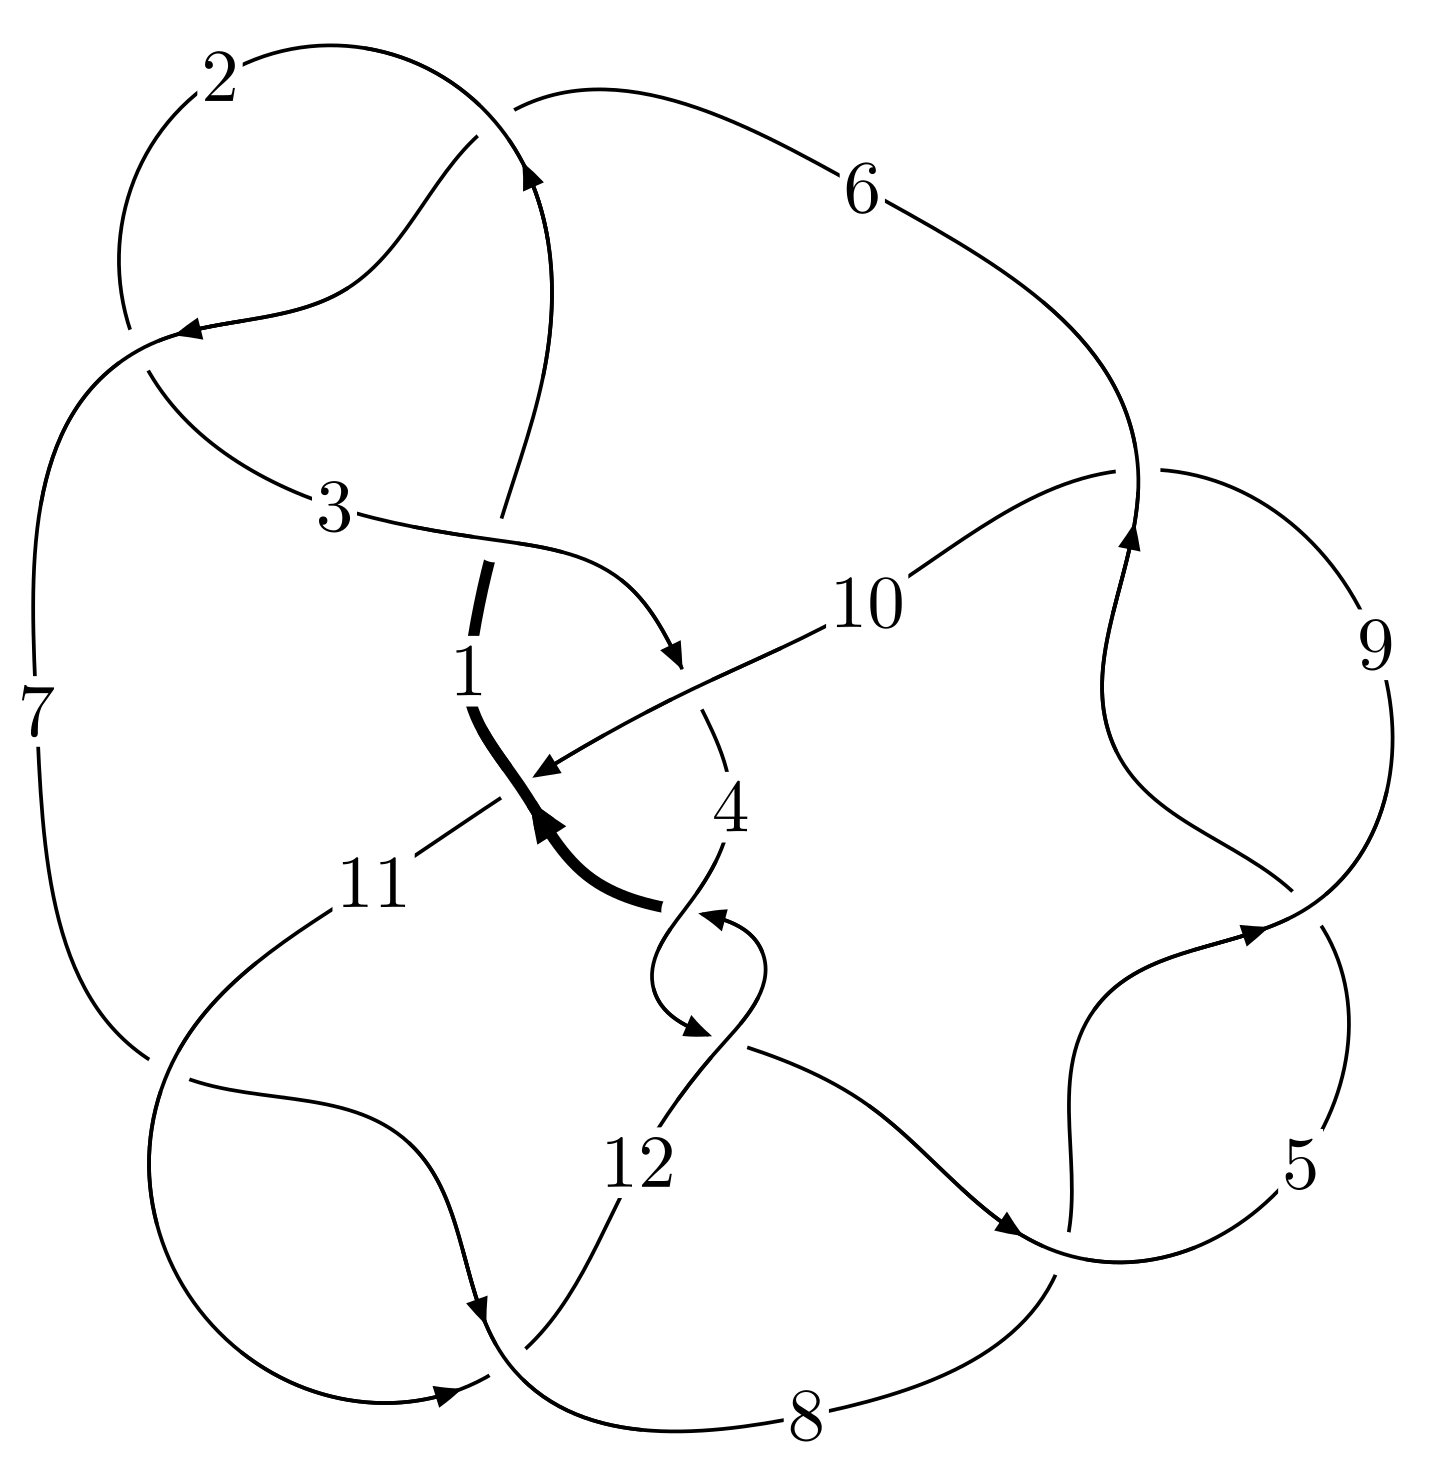
\includegraphics[width=112pt]{../../../GIT/diagram.site/Diagrams/png/1461_12a_0660.png}\\
\ \ \ A knot diagram\footnotemark}&
\allowdisplaybreaks
\textbf{Linearized knot diagam} \\
\cline{2-2}
 &
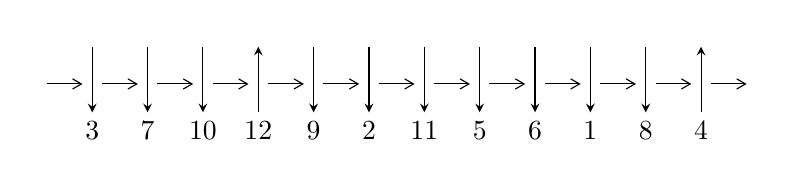
\begin{tikzpicture}[x=20pt, y=17pt]
	% nodes
	\node (C0) at (0, 0) {};
	\node (C1) at (1, 0) {};
	\node (C1U) at (1, +1) {};
	\node (C1D) at (1, -1) {3};

	\node (C2) at (2, 0) {};
	\node (C2U) at (2, +1) {};
	\node (C2D) at (2, -1) {7};

	\node (C3) at (3, 0) {};
	\node (C3U) at (3, +1) {};
	\node (C3D) at (3, -1) {10};

	\node (C4) at (4, 0) {};
	\node (C4U) at (4, +1) {};
	\node (C4D) at (4, -1) {12};

	\node (C5) at (5, 0) {};
	\node (C5U) at (5, +1) {};
	\node (C5D) at (5, -1) {9};

	\node (C6) at (6, 0) {};
	\node (C6U) at (6, +1) {};
	\node (C6D) at (6, -1) {2};

	\node (C7) at (7, 0) {};
	\node (C7U) at (7, +1) {};
	\node (C7D) at (7, -1) {11};

	\node (C8) at (8, 0) {};
	\node (C8U) at (8, +1) {};
	\node (C8D) at (8, -1) {5};

	\node (C9) at (9, 0) {};
	\node (C9U) at (9, +1) {};
	\node (C9D) at (9, -1) {6};

	\node (C10) at (10, 0) {};
	\node (C10U) at (10, +1) {};
	\node (C10D) at (10, -1) {1};

	\node (C11) at (11, 0) {};
	\node (C11U) at (11, +1) {};
	\node (C11D) at (11, -1) {8};

	\node (C12) at (12, 0) {};
	\node (C12U) at (12, +1) {};
	\node (C12D) at (12, -1) {4};
	\node (C13) at (13, 0) {};

	% arrows
	\draw[->,>={angle 60}]
	(C0) edge (C1) (C1) edge (C2) (C2) edge (C3) (C3) edge (C4) (C4) edge (C5) (C5) edge (C6) (C6) edge (C7) (C7) edge (C8) (C8) edge (C9) (C9) edge (C10) (C10) edge (C11) (C11) edge (C12) (C12) edge (C13) ;	\draw[->,>=stealth]
	(C1U) edge (C1D) (C2U) edge (C2D) (C3U) edge (C3D) (C4D) edge (C4U) (C5U) edge (C5D) (C6U) edge (C6D) (C7U) edge (C7D) (C8U) edge (C8D) (C9U) edge (C9D) (C10U) edge (C10D) (C11U) edge (C11D) (C12D) edge (C12U) ;
	\end{tikzpicture} \\
\hhline{~~} \\& 
\textbf{Solving Sequence} \\ \cline{2-2} 
 &
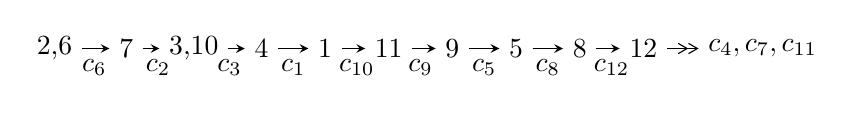
\begin{tikzpicture}[x=23pt, y=7pt]
	% node
	\node (A0) at (-1/8, 0) {2,6};
	\node (A1) at (1, 0) {7};
	\node (A2) at (33/16, 0) {3,10};
	\node (A3) at (25/8, 0) {4};
	\node (A4) at (33/8, 0) {1};
	\node (A5) at (41/8, 0) {11};
	\node (A6) at (49/8, 0) {9};
	\node (A7) at (57/8, 0) {5};
	\node (A8) at (65/8, 0) {8};
	\node (A9) at (73/8, 0) {12};
	\node (C1) at (1/2, -1) {$c_{6}$};
	\node (C2) at (3/2, -1) {$c_{2}$};
	\node (C3) at (21/8, -1) {$c_{3}$};
	\node (C4) at (29/8, -1) {$c_{1}$};
	\node (C5) at (37/8, -1) {$c_{10}$};
	\node (C6) at (45/8, -1) {$c_{9}$};
	\node (C7) at (53/8, -1) {$c_{5}$};
	\node (C8) at (61/8, -1) {$c_{8}$};
	\node (C9) at (69/8, -1) {$c_{12}$};
	\node (A10) at (11, 0) {$c_{4},c_{7},c_{11}$};

	% edge
	\draw[->,>=stealth]	
	(A0) edge (A1) (A1) edge (A2) (A2) edge (A3) (A3) edge (A4) (A4) edge (A5) (A5) edge (A6) (A6) edge (A7) (A7) edge (A8) (A8) edge (A9) ;
	\draw[->>,>={angle 60}]	
	(A9) edge (A10);
\end{tikzpicture} \\ 

\end{tabular} \\

\footnotetext{
The image of knot diagram is generated by the software ``\textbf{Draw programme}" developed by Andrew Bartholomew(\url{http://www.layer8.co.uk/maths/draw/index.htm\#Running-draw}), where we modified some parts for our purpose(\url{https://github.com/CATsTAILs/LinksPainter}).
}\phantom \\ \newline 
\centering \textbf{Ideals for irreducible components\footnotemark of $X_{\text{par}}$} 
 
\begin{align*}
I^u_{1}&=\langle 
8.15678\times10^{158} u^{106}+3.46027\times10^{159} u^{105}+\cdots+1.38526\times10^{159} b-1.85181\times10^{159},\\
\phantom{I^u_{1}}&\phantom{= \langle  }8.94370\times10^{158} u^{106}+2.49875\times10^{159} u^{105}+\cdots+1.38526\times10^{159} a-5.17367\times10^{158},\;u^{107}+3 u^{106}+\cdots- u+1\rangle \\
I^u_{2}&=\langle 
-334 u^{25}+695 u^{24}+\cdots+299 b+422,\;-1077 u^{25}+1225 u^{24}+\cdots+299 a-478,\\
\phantom{I^u_{2}}&\phantom{= \langle  }u^{26}-7 u^{24}+\cdots+2 u+1\rangle \\
\\
\end{align*}
\raggedright * 2 irreducible components of $\dim_{\mathbb{C}}=0$, with total 133 representations.\\
\footnotetext{All coefficients of polynomials are rational numbers. But the coefficients are sometimes approximated in decimal forms when there is not enough margin.}
\newpage
\renewcommand{\arraystretch}{1}
\centering \section*{I. $I^u_{1}= \langle 8.16\times10^{158} u^{106}+3.46\times10^{159} u^{105}+\cdots+1.39\times10^{159} b-1.85\times10^{159},\;8.94\times10^{158} u^{106}+2.50\times10^{159} u^{105}+\cdots+1.39\times10^{159} a-5.17\times10^{158},\;u^{107}+3 u^{106}+\cdots- u+1 \rangle$}
\flushleft \textbf{(i) Arc colorings}\\
\begin{tabular}{m{7pt} m{180pt} m{7pt} m{180pt} }
\flushright $a_{2}=$&$\begin{pmatrix}0\\u\end{pmatrix}$ \\
\flushright $a_{6}=$&$\begin{pmatrix}1\\0\end{pmatrix}$ \\
\flushright $a_{7}=$&$\begin{pmatrix}1\\u^2\end{pmatrix}$ \\
\flushright $a_{3}=$&$\begin{pmatrix}- u\\- u^3+u\end{pmatrix}$ \\
\flushright $a_{10}=$&$\begin{pmatrix}-0.645634 u^{106}-1.80382 u^{105}+\cdots+0.670204 u+0.373480\\-0.588827 u^{106}-2.49792 u^{105}+\cdots+3.21354 u+1.33680\end{pmatrix}$ \\
\flushright $a_{4}=$&$\begin{pmatrix}0.502479 u^{106}+2.01864 u^{105}+\cdots-10.0754 u+2.39998\\0.0132447 u^{106}-0.404849 u^{105}+\cdots+3.43356 u+0.0731468\end{pmatrix}$ \\
\flushright $a_{1}=$&$\begin{pmatrix}u^3\\u^5- u^3+u\end{pmatrix}$ \\
\flushright $a_{11}=$&$\begin{pmatrix}-0.676399 u^{106}-1.47429 u^{105}+\cdots+0.764777 u+0.210767\\-0.903755 u^{106}-2.97696 u^{105}+\cdots+3.70148 u+0.712057\end{pmatrix}$ \\
\flushright $a_{9}=$&$\begin{pmatrix}-1.23446 u^{106}-4.30174 u^{105}+\cdots+3.88374 u+1.71028\\-0.588827 u^{106}-2.49792 u^{105}+\cdots+3.21354 u+1.33680\end{pmatrix}$ \\
\flushright $a_{5}=$&$\begin{pmatrix}-1.74790 u^{106}-3.18997 u^{105}+\cdots+0.252284 u+1.44174\\-1.10312 u^{106}-3.32060 u^{105}+\cdots+3.24796 u+0.488580\end{pmatrix}$ \\
\flushright $a_{8}=$&$\begin{pmatrix}0.623400 u^{106}+1.53441 u^{105}+\cdots+3.10548 u+0.978324\\0.207767 u^{106}+1.77731 u^{105}+\cdots-0.844158 u-1.08994\end{pmatrix}$ \\
\flushright $a_{12}=$&$\begin{pmatrix}3.48966 u^{106}+10.9581 u^{105}+\cdots-1.32391 u-0.827989\\-0.527015 u^{106}+0.370912 u^{105}+\cdots+3.18338 u-2.35468\end{pmatrix}$\\&\end{tabular}
\flushleft \textbf{(ii) Obstruction class $= -1$}\\~\\
\flushleft \textbf{(iii) Cusp Shapes $= 1.99910 u^{106}+5.78442 u^{105}+\cdots-1.90938 u-13.0241$}\\~\\
\newpage\renewcommand{\arraystretch}{1}
\flushleft \textbf{(iv) u-Polynomials at the component}\newline \\
\begin{tabular}{m{50pt}|m{274pt}}
Crossings & \hspace{64pt}u-Polynomials at each crossing \\
\hline $$\begin{aligned}c_{1}\end{aligned}$$&$\begin{aligned}
&u^{107}+51 u^{106}+\cdots+27 u+1
\end{aligned}$\\
\hline $$\begin{aligned}c_{2},c_{6}\end{aligned}$$&$\begin{aligned}
&u^{107}-3 u^{106}+\cdots- u-1
\end{aligned}$\\
\hline $$\begin{aligned}c_{3}\end{aligned}$$&$\begin{aligned}
&u^{107}+2 u^{106}+\cdots+55540 u+8117
\end{aligned}$\\
\hline $$\begin{aligned}c_{4},c_{12}\end{aligned}$$&$\begin{aligned}
&u^{107}+6 u^{106}+\cdots+63 u+1
\end{aligned}$\\
\hline $$\begin{aligned}c_{5},c_{8},c_{9}\end{aligned}$$&$\begin{aligned}
&u^{107}+3 u^{106}+\cdots+3214 u-319
\end{aligned}$\\
\hline $$\begin{aligned}c_{7},c_{11}\end{aligned}$$&$\begin{aligned}
&u^{107}-3 u^{106}+\cdots-20005 u-18299
\end{aligned}$\\
\hline $$\begin{aligned}c_{10}\end{aligned}$$&$\begin{aligned}
&u^{107}-13 u^{106}+\cdots+650 u-113
\end{aligned}$\\
\hline
\end{tabular}\\~\\
\newpage\renewcommand{\arraystretch}{1}
\flushleft \textbf{(v) Riley Polynomials at the component}\newline \\
\begin{tabular}{m{50pt}|m{274pt}}
Crossings & \hspace{64pt}Riley Polynomials at each crossing \\
\hline $$\begin{aligned}c_{1}\end{aligned}$$&$\begin{aligned}
&y^{107}+25 y^{106}+\cdots-85 y-1
\end{aligned}$\\
\hline $$\begin{aligned}c_{2},c_{6}\end{aligned}$$&$\begin{aligned}
&y^{107}-51 y^{106}+\cdots+27 y-1
\end{aligned}$\\
\hline $$\begin{aligned}c_{3}\end{aligned}$$&$\begin{aligned}
&y^{107}-22 y^{106}+\cdots+3840497938 y-65885689
\end{aligned}$\\
\hline $$\begin{aligned}c_{4},c_{12}\end{aligned}$$&$\begin{aligned}
&y^{107}+102 y^{106}+\cdots+679 y-1
\end{aligned}$\\
\hline $$\begin{aligned}c_{5},c_{8},c_{9}\end{aligned}$$&$\begin{aligned}
&y^{107}-119 y^{106}+\cdots+4129712 y-101761
\end{aligned}$\\
\hline $$\begin{aligned}c_{7},c_{11}\end{aligned}$$&$\begin{aligned}
&y^{107}-101 y^{106}+\cdots+8587611801 y-334853401
\end{aligned}$\\
\hline $$\begin{aligned}c_{10}\end{aligned}$$&$\begin{aligned}
&y^{107}-19 y^{106}+\cdots+1683354 y-12769
\end{aligned}$\\
\hline
\end{tabular}\\~\\
\newpage\flushleft \textbf{(vi) Complex Volumes and Cusp Shapes}
$$\begin{array}{c|c|c}  
\text{Solutions to }I^u_{1}& \I (\text{vol} + \sqrt{-1}CS) & \text{Cusp shape}\\
 \hline 
\begin{aligned}
u &= -0.961830 + 0.332422 I \\
a &= -0.95342 - 1.48514 I \\
b &= -0.213133 + 0.493321 I\end{aligned}
 & -3.29063 + 1.20407 I & \phantom{-0.000000 } 0 \\ \hline\begin{aligned}
u &= -0.961830 - 0.332422 I \\
a &= -0.95342 + 1.48514 I \\
b &= -0.213133 - 0.493321 I\end{aligned}
 & -3.29063 - 1.20407 I & \phantom{-0.000000 } 0 \\ \hline\begin{aligned}
u &= \phantom{-}0.958742 + 0.341227 I \\
a &= -1.08709 + 2.34096 I \\
b &= -0.217132 + 0.274273 I\end{aligned}
 & -7.34857 - 1.24944 I & \phantom{-0.000000 } 0 \\ \hline\begin{aligned}
u &= \phantom{-}0.958742 - 0.341227 I \\
a &= -1.08709 - 2.34096 I \\
b &= -0.217132 - 0.274273 I\end{aligned}
 & -7.34857 + 1.24944 I & \phantom{-0.000000 } 0 \\ \hline\begin{aligned}
u &= -0.369587 + 0.955253 I \\
a &= \phantom{-}0.870511 + 0.620617 I \\
b &= -1.61405 - 0.28862 I\end{aligned}
 & -12.0819 - 11.6140 I & \phantom{-0.000000 } 0 \\ \hline\begin{aligned}
u &= -0.369587 - 0.955253 I \\
a &= \phantom{-}0.870511 - 0.620617 I \\
b &= -1.61405 + 0.28862 I\end{aligned}
 & -12.0819 + 11.6140 I & \phantom{-0.000000 } 0 \\ \hline\begin{aligned}
u &= -0.499372 + 0.834983 I \\
a &= -1.168340 + 0.353127 I \\
b &= \phantom{-}1.47972 + 0.06590 I\end{aligned}
 & -6.32317 + 1.20142 I & \phantom{-0.000000 } 0 \\ \hline\begin{aligned}
u &= -0.499372 - 0.834983 I \\
a &= -1.168340 - 0.353127 I \\
b &= \phantom{-}1.47972 - 0.06590 I\end{aligned}
 & -6.32317 - 1.20142 I & \phantom{-0.000000 } 0 \\ \hline\begin{aligned}
u &= -0.946435 + 0.223421 I \\
a &= \phantom{-}0.538397 - 0.647153 I \\
b &= \phantom{-}0.705787 + 0.351906 I\end{aligned}
 & -3.77086 - 1.62099 I & \phantom{-0.000000 } 0 \\ \hline\begin{aligned}
u &= -0.946435 - 0.223421 I \\
a &= \phantom{-}0.538397 + 0.647153 I \\
b &= \phantom{-}0.705787 - 0.351906 I\end{aligned}
 & -3.77086 + 1.62099 I & \phantom{-0.000000 } 0\\
 \hline 
 \end{array}$$\newpage$$\begin{array}{c|c|c}  
\text{Solutions to }I^u_{1}& \I (\text{vol} + \sqrt{-1}CS) & \text{Cusp shape}\\
 \hline 
\begin{aligned}
u &= \phantom{-}0.847260 + 0.476918 I \\
a &= -0.344512 + 0.224684 I \\
b &= \phantom{-}0.745400 - 0.353078 I\end{aligned}
 & -0.307193 - 0.490634 I & \phantom{-0.000000 } 0 \\ \hline\begin{aligned}
u &= \phantom{-}0.847260 - 0.476918 I \\
a &= -0.344512 - 0.224684 I \\
b &= \phantom{-}0.745400 + 0.353078 I\end{aligned}
 & -0.307193 + 0.490634 I & \phantom{-0.000000 } 0 \\ \hline\begin{aligned}
u &= \phantom{-}0.798708 + 0.542944 I \\
a &= -0.14181 + 1.61061 I \\
b &= -0.991529 - 0.249020 I\end{aligned}
 & -0.18748 - 3.71647 I & \phantom{-0.000000 } 0 \\ \hline\begin{aligned}
u &= \phantom{-}0.798708 - 0.542944 I \\
a &= -0.14181 - 1.61061 I \\
b &= -0.991529 + 0.249020 I\end{aligned}
 & -0.18748 + 3.71647 I & \phantom{-0.000000 } 0 \\ \hline\begin{aligned}
u &= \phantom{-}0.998931 + 0.309324 I \\
a &= -1.28251 + 1.21264 I \\
b &= -0.254601 - 1.213830 I\end{aligned}
 & -7.79059 - 0.96657 I & \phantom{-0.000000 } 0 \\ \hline\begin{aligned}
u &= \phantom{-}0.998931 - 0.309324 I \\
a &= -1.28251 - 1.21264 I \\
b &= -0.254601 + 1.213830 I\end{aligned}
 & -7.79059 + 0.96657 I & \phantom{-0.000000 } 0 \\ \hline\begin{aligned}
u &= \phantom{-}0.413338 + 0.837059 I \\
a &= -0.713227 + 1.169820 I \\
b &= \phantom{-}0.677392 - 0.896334 I\end{aligned}
 & -4.53636 + 7.22884 I & \phantom{-0.000000 } 0 \\ \hline\begin{aligned}
u &= \phantom{-}0.413338 - 0.837059 I \\
a &= -0.713227 - 1.169820 I \\
b &= \phantom{-}0.677392 + 0.896334 I\end{aligned}
 & -4.53636 - 7.22884 I & \phantom{-0.000000 } 0 \\ \hline\begin{aligned}
u &= \phantom{-}0.975496 + 0.451189 I \\
a &= \phantom{-}0.195028 - 0.866105 I \\
b &= \phantom{-}0.265652 + 0.588887 I\end{aligned}
 & -2.30476 - 1.54496 I & \phantom{-0.000000 } 0 \\ \hline\begin{aligned}
u &= \phantom{-}0.975496 - 0.451189 I \\
a &= \phantom{-}0.195028 + 0.866105 I \\
b &= \phantom{-}0.265652 - 0.588887 I\end{aligned}
 & -2.30476 + 1.54496 I & \phantom{-0.000000 } 0\\
 \hline 
 \end{array}$$\newpage$$\begin{array}{c|c|c}  
\text{Solutions to }I^u_{1}& \I (\text{vol} + \sqrt{-1}CS) & \text{Cusp shape}\\
 \hline 
\begin{aligned}
u &= -0.355666 + 0.853164 I \\
a &= -0.200155 - 0.729502 I \\
b &= \phantom{-}0.362854 + 0.444344 I\end{aligned}
 & \phantom{-}0.88775 - 3.04504 I & \phantom{-0.000000 } 0 \\ \hline\begin{aligned}
u &= -0.355666 - 0.853164 I \\
a &= -0.200155 + 0.729502 I \\
b &= \phantom{-}0.362854 - 0.444344 I\end{aligned}
 & \phantom{-}0.88775 + 3.04504 I & \phantom{-0.000000 } 0 \\ \hline\begin{aligned}
u &= -0.983341 + 0.443642 I \\
a &= -0.656672 - 0.590776 I \\
b &= \phantom{-}0.763728 + 0.511598 I\end{aligned}
 & -2.44654 + 4.26744 I & \phantom{-0.000000 } 0 \\ \hline\begin{aligned}
u &= -0.983341 - 0.443642 I \\
a &= -0.656672 + 0.590776 I \\
b &= \phantom{-}0.763728 - 0.511598 I\end{aligned}
 & -2.44654 - 4.26744 I & \phantom{-0.000000 } 0 \\ \hline\begin{aligned}
u &= -0.467684 + 0.792634 I \\
a &= -1.24282 - 0.75290 I \\
b &= \phantom{-}1.51899 + 0.09496 I\end{aligned}
 & -6.46974 - 4.55544 I & \phantom{-0.000000 } 0 \\ \hline\begin{aligned}
u &= -0.467684 - 0.792634 I \\
a &= -1.24282 + 0.75290 I \\
b &= \phantom{-}1.51899 - 0.09496 I\end{aligned}
 & -6.46974 + 4.55544 I & \phantom{-0.000000 } 0 \\ \hline\begin{aligned}
u &= \phantom{-}1.082590 + 0.029157 I \\
a &= -0.991798 + 0.623311 I \\
b &= -1.62910 - 0.03464 I\end{aligned}
 & -11.97000 - 2.95811 I & \phantom{-0.000000 } 0 \\ \hline\begin{aligned}
u &= \phantom{-}1.082590 - 0.029157 I \\
a &= -0.991798 - 0.623311 I \\
b &= -1.62910 + 0.03464 I\end{aligned}
 & -11.97000 + 2.95811 I & \phantom{-0.000000 } 0 \\ \hline\begin{aligned}
u &= \phantom{-}0.401674 + 0.819898 I \\
a &= -0.755345 + 0.515225 I \\
b &= \phantom{-}1.271110 - 0.201930 I\end{aligned}
 & -1.60802 + 2.19584 I & \phantom{-0.000000 } 0 \\ \hline\begin{aligned}
u &= \phantom{-}0.401674 - 0.819898 I \\
a &= -0.755345 - 0.515225 I \\
b &= \phantom{-}1.271110 + 0.201930 I\end{aligned}
 & -1.60802 - 2.19584 I & \phantom{-0.000000 } 0\\
 \hline 
 \end{array}$$\newpage$$\begin{array}{c|c|c}  
\text{Solutions to }I^u_{1}& \I (\text{vol} + \sqrt{-1}CS) & \text{Cusp shape}\\
 \hline 
\begin{aligned}
u &= \phantom{-}0.646248 + 0.881601 I \\
a &= -0.254328 - 0.603168 I \\
b &= \phantom{-}0.348185 + 0.570605 I\end{aligned}
 & -3.33409 - 3.47498 I & \phantom{-0.000000 } 0 \\ \hline\begin{aligned}
u &= \phantom{-}0.646248 - 0.881601 I \\
a &= -0.254328 + 0.603168 I \\
b &= \phantom{-}0.348185 - 0.570605 I\end{aligned}
 & -3.33409 + 3.47498 I & \phantom{-0.000000 } 0 \\ \hline\begin{aligned}
u &= \phantom{-}0.261399 + 1.062550 I \\
a &= \phantom{-}0.487280 - 0.288942 I \\
b &= -1.50275 + 0.10870 I\end{aligned}
 & -5.36658 + 4.88981 I & \phantom{-0.000000 } 0 \\ \hline\begin{aligned}
u &= \phantom{-}0.261399 - 1.062550 I \\
a &= \phantom{-}0.487280 + 0.288942 I \\
b &= -1.50275 - 0.10870 I\end{aligned}
 & -5.36658 - 4.88981 I & \phantom{-0.000000 } 0 \\ \hline\begin{aligned}
u &= \phantom{-}1.023000 + 0.428534 I \\
a &= \phantom{-}2.53956 - 0.97539 I \\
b &= \phantom{-}1.59921 + 0.09408 I\end{aligned}
 & -13.7231 - 6.2790 I & \phantom{-0.000000 } 0 \\ \hline\begin{aligned}
u &= \phantom{-}1.023000 - 0.428534 I \\
a &= \phantom{-}2.53956 + 0.97539 I \\
b &= \phantom{-}1.59921 - 0.09408 I\end{aligned}
 & -13.7231 + 6.2790 I & \phantom{-0.000000 } 0 \\ \hline\begin{aligned}
u &= -0.589912 + 0.656621 I \\
a &= \phantom{-}0.437981 + 1.143260 I \\
b &= -0.087007 - 0.593363 I\end{aligned}
 & \phantom{-}2.54220 + 0.64997 I & \phantom{-0.000000 } 0 \\ \hline\begin{aligned}
u &= -0.589912 - 0.656621 I \\
a &= \phantom{-}0.437981 - 1.143260 I \\
b &= -0.087007 + 0.593363 I\end{aligned}
 & \phantom{-}2.54220 - 0.64997 I & \phantom{-0.000000 } 0 \\ \hline\begin{aligned}
u &= -1.043800 + 0.426405 I \\
a &= \phantom{-}1.20392 + 0.88892 I \\
b &= \phantom{-}1.60785 + 0.07237 I\end{aligned}
 & -9.62067 + 2.93444 I & \phantom{-0.000000 } 0 \\ \hline\begin{aligned}
u &= -1.043800 - 0.426405 I \\
a &= \phantom{-}1.20392 - 0.88892 I \\
b &= \phantom{-}1.60785 - 0.07237 I\end{aligned}
 & -9.62067 - 2.93444 I & \phantom{-0.000000 } 0\\
 \hline 
 \end{array}$$\newpage$$\begin{array}{c|c|c}  
\text{Solutions to }I^u_{1}& \I (\text{vol} + \sqrt{-1}CS) & \text{Cusp shape}\\
 \hline 
\begin{aligned}
u &= -1.12940\phantom{ +0.000000I} \\
a &= -1.00887\phantom{ +0.000000I} \\
b &= -1.42458\phantom{ +0.000000I}\end{aligned}
 & -7.23387\phantom{ +0.000000I} & \phantom{-0.000000 } 0 \\ \hline\begin{aligned}
u &= -1.035950 + 0.471098 I \\
a &= \phantom{-}0.99679 + 3.24691 I \\
b &= \phantom{-}1.50492 + 0.07277 I\end{aligned}
 & -13.41210 + 0.09296 I & \phantom{-0.000000 } 0 \\ \hline\begin{aligned}
u &= -1.035950 - 0.471098 I \\
a &= \phantom{-}0.99679 - 3.24691 I \\
b &= \phantom{-}1.50492 - 0.07277 I\end{aligned}
 & -13.41210 - 0.09296 I & \phantom{-0.000000 } 0 \\ \hline\begin{aligned}
u &= \phantom{-}1.059380 + 0.421034 I \\
a &= \phantom{-}0.192519 - 0.909579 I \\
b &= \phantom{-}1.79206 - 0.30617 I\end{aligned}
 & -14.4279 + 0.5275 I & \phantom{-0.000000 } 0 \\ \hline\begin{aligned}
u &= \phantom{-}1.059380 - 0.421034 I \\
a &= \phantom{-}0.192519 + 0.909579 I \\
b &= \phantom{-}1.79206 + 0.30617 I\end{aligned}
 & -14.4279 - 0.5275 I & \phantom{-0.000000 } 0 \\ \hline\begin{aligned}
u &= \phantom{-}1.053830 + 0.463544 I \\
a &= \phantom{-}0.59344 - 2.50820 I \\
b &= \phantom{-}1.51988 + 0.16655 I\end{aligned}
 & -9.35195 - 3.71564 I & \phantom{-0.000000 } 0 \\ \hline\begin{aligned}
u &= \phantom{-}1.053830 - 0.463544 I \\
a &= \phantom{-}0.59344 + 2.50820 I \\
b &= \phantom{-}1.51988 - 0.16655 I\end{aligned}
 & -9.35195 + 3.71564 I & \phantom{-0.000000 } 0 \\ \hline\begin{aligned}
u &= -1.027130 + 0.527139 I \\
a &= -1.39492 - 0.38480 I \\
b &= -0.661152 + 0.306944 I\end{aligned}
 & -5.95960 + 4.75876 I & \phantom{-0.000000 } 0 \\ \hline\begin{aligned}
u &= -1.027130 - 0.527139 I \\
a &= -1.39492 + 0.38480 I \\
b &= -0.661152 - 0.306944 I\end{aligned}
 & -5.95960 - 4.75876 I & \phantom{-0.000000 } 0 \\ \hline\begin{aligned}
u &= -1.001470 + 0.576910 I \\
a &= \phantom{-}0.512781 + 1.161960 I \\
b &= \phantom{-}0.239029 - 0.663644 I\end{aligned}
 & \phantom{-}1.30721 + 4.16361 I & \phantom{-0.000000 } 0\\
 \hline 
 \end{array}$$\newpage$$\begin{array}{c|c|c}  
\text{Solutions to }I^u_{1}& \I (\text{vol} + \sqrt{-1}CS) & \text{Cusp shape}\\
 \hline 
\begin{aligned}
u &= -1.001470 - 0.576910 I \\
a &= \phantom{-}0.512781 - 1.161960 I \\
b &= \phantom{-}0.239029 + 0.663644 I\end{aligned}
 & \phantom{-}1.30721 - 4.16361 I & \phantom{-0.000000 } 0 \\ \hline\begin{aligned}
u &= -1.069050 + 0.460268 I \\
a &= \phantom{-}0.32136 + 2.22693 I \\
b &= \phantom{-}1.67047 - 0.46711 I\end{aligned}
 & -14.1458 + 7.4015 I & \phantom{-0.000000 } 0 \\ \hline\begin{aligned}
u &= -1.069050 - 0.460268 I \\
a &= \phantom{-}0.32136 - 2.22693 I \\
b &= \phantom{-}1.67047 + 0.46711 I\end{aligned}
 & -14.1458 - 7.4015 I & \phantom{-0.000000 } 0 \\ \hline\begin{aligned}
u &= -0.752673 + 0.357367 I \\
a &= -0.82907 - 2.31432 I \\
b &= -0.962388 + 0.289012 I\end{aligned}
 & -1.52828 - 0.85653 I & -15.4191 - 2.9581 I \\ \hline\begin{aligned}
u &= -0.752673 - 0.357367 I \\
a &= -0.82907 + 2.31432 I \\
b &= -0.962388 - 0.289012 I\end{aligned}
 & -1.52828 + 0.85653 I & -15.4191 + 2.9581 I \\ \hline\begin{aligned}
u &= \phantom{-}1.035010 + 0.557185 I \\
a &= \phantom{-}0.160485 - 0.131907 I \\
b &= -0.630787 + 0.508665 I\end{aligned}
 & -1.66121 - 4.79673 I & \phantom{-0.000000 } 0 \\ \hline\begin{aligned}
u &= \phantom{-}1.035010 - 0.557185 I \\
a &= \phantom{-}0.160485 + 0.131907 I \\
b &= -0.630787 - 0.508665 I\end{aligned}
 & -1.66121 + 4.79673 I & \phantom{-0.000000 } 0 \\ \hline\begin{aligned}
u &= -1.178020 + 0.076352 I \\
a &= -0.015667 - 0.228494 I \\
b &= -0.811495 - 0.658408 I\end{aligned}
 & -10.09900 - 4.81161 I & \phantom{-0.000000 } 0 \\ \hline\begin{aligned}
u &= -1.178020 - 0.076352 I \\
a &= -0.015667 + 0.228494 I \\
b &= -0.811495 + 0.658408 I\end{aligned}
 & -10.09900 + 4.81161 I & \phantom{-0.000000 } 0 \\ \hline\begin{aligned}
u &= \phantom{-}0.544622 + 0.609128 I \\
a &= \phantom{-}0.012491 - 0.923495 I \\
b &= \phantom{-}0.734322 + 0.303158 I\end{aligned}
 & -0.166974 + 0.153852 I & -8.00000 + 2.06306 I\\
 \hline 
 \end{array}$$\newpage$$\begin{array}{c|c|c}  
\text{Solutions to }I^u_{1}& \I (\text{vol} + \sqrt{-1}CS) & \text{Cusp shape}\\
 \hline 
\begin{aligned}
u &= \phantom{-}0.544622 - 0.609128 I \\
a &= \phantom{-}0.012491 + 0.923495 I \\
b &= \phantom{-}0.734322 - 0.303158 I\end{aligned}
 & -0.166974 - 0.153852 I & -8.00000 - 2.06306 I \\ \hline\begin{aligned}
u &= \phantom{-}1.042950 + 0.564382 I \\
a &= \phantom{-}0.30084 - 1.66219 I \\
b &= \phantom{-}0.444295 + 0.476539 I\end{aligned}
 & -1.60574 - 7.73159 I & \phantom{-0.000000 } 0 \\ \hline\begin{aligned}
u &= \phantom{-}1.042950 - 0.564382 I \\
a &= \phantom{-}0.30084 + 1.66219 I \\
b &= \phantom{-}0.444295 - 0.476539 I\end{aligned}
 & -1.60574 + 7.73159 I & \phantom{-0.000000 } 0 \\ \hline\begin{aligned}
u &= -1.063710 + 0.548200 I \\
a &= \phantom{-}0.932445 + 0.402901 I \\
b &= -0.650175 - 1.199090 I\end{aligned}
 & -6.09234 + 5.54333 I & \phantom{-0.000000 } 0 \\ \hline\begin{aligned}
u &= -1.063710 - 0.548200 I \\
a &= \phantom{-}0.932445 - 0.402901 I \\
b &= -0.650175 + 1.199090 I\end{aligned}
 & -6.09234 - 5.54333 I & \phantom{-0.000000 } 0 \\ \hline\begin{aligned}
u &= \phantom{-}0.482974 + 0.625314 I \\
a &= \phantom{-}0.80091 - 1.39267 I \\
b &= -0.390008 + 0.344012 I\end{aligned}
 & \phantom{-}0.02557 + 3.02324 I & -6.28635 - 4.37518 I \\ \hline\begin{aligned}
u &= \phantom{-}0.482974 - 0.625314 I \\
a &= \phantom{-}0.80091 + 1.39267 I \\
b &= -0.390008 - 0.344012 I\end{aligned}
 & \phantom{-}0.02557 - 3.02324 I & -6.28635 + 4.37518 I \\ \hline\begin{aligned}
u &= -0.428679 + 0.620294 I \\
a &= \phantom{-}0.26578 + 1.93424 I \\
b &= \phantom{-}0.638474 - 1.006270 I\end{aligned}
 & -4.25310 - 0.91402 I & -12.05109 + 0.86644 I \\ \hline\begin{aligned}
u &= -0.428679 - 0.620294 I \\
a &= \phantom{-}0.26578 - 1.93424 I \\
b &= \phantom{-}0.638474 + 1.006270 I\end{aligned}
 & -4.25310 + 0.91402 I & -12.05109 - 0.86644 I \\ \hline\begin{aligned}
u &= -1.086820 + 0.616697 I \\
a &= \phantom{-}0.05129 - 2.46156 I \\
b &= -1.53726 + 0.13189 I\end{aligned}
 & -8.32326 + 9.85252 I & \phantom{-0.000000 } 0\\
 \hline 
 \end{array}$$\newpage$$\begin{array}{c|c|c}  
\text{Solutions to }I^u_{1}& \I (\text{vol} + \sqrt{-1}CS) & \text{Cusp shape}\\
 \hline 
\begin{aligned}
u &= -1.086820 - 0.616697 I \\
a &= \phantom{-}0.05129 + 2.46156 I \\
b &= -1.53726 - 0.13189 I\end{aligned}
 & -8.32326 - 9.85252 I & \phantom{-0.000000 } 0 \\ \hline\begin{aligned}
u &= \phantom{-}1.110860 + 0.607119 I \\
a &= -0.29657 + 1.87350 I \\
b &= -1.359380 - 0.262195 I\end{aligned}
 & -3.71417 - 7.50040 I & \phantom{-0.000000 } 0 \\ \hline\begin{aligned}
u &= \phantom{-}1.110860 - 0.607119 I \\
a &= -0.29657 - 1.87350 I \\
b &= -1.359380 + 0.262195 I\end{aligned}
 & -3.71417 + 7.50040 I & \phantom{-0.000000 } 0 \\ \hline\begin{aligned}
u &= \phantom{-}1.120690 + 0.617015 I \\
a &= -0.70783 + 1.44475 I \\
b &= -0.757046 - 0.975658 I\end{aligned}
 & -6.6596 - 12.6316 I & \phantom{-0.000000 } 0 \\ \hline\begin{aligned}
u &= \phantom{-}1.120690 - 0.617015 I \\
a &= -0.70783 - 1.44475 I \\
b &= -0.757046 + 0.975658 I\end{aligned}
 & -6.6596 + 12.6316 I & \phantom{-0.000000 } 0 \\ \hline\begin{aligned}
u &= \phantom{-}1.27963\phantom{ +0.000000I} \\
a &= -0.0992902\phantom{ +0.000000I} \\
b &= -0.553045\phantom{ +0.000000I}\end{aligned}
 & -5.05733\phantom{ +0.000000I} & \phantom{-0.000000 } 0 \\ \hline\begin{aligned}
u &= \phantom{-}0.701738 + 0.120348 I \\
a &= -1.46299 - 1.49108 I \\
b &= -1.64323 + 0.14164 I\end{aligned}
 & -12.19130 + 3.25713 I & -15.3274 - 4.1847 I \\ \hline\begin{aligned}
u &= \phantom{-}0.701738 - 0.120348 I \\
a &= -1.46299 + 1.49108 I \\
b &= -1.64323 - 0.14164 I\end{aligned}
 & -12.19130 - 3.25713 I & -15.3274 + 4.1847 I \\ \hline\begin{aligned}
u &= -1.134770 + 0.612321 I \\
a &= -0.447512 - 1.033430 I \\
b &= -0.511287 + 0.526545 I\end{aligned}
 & -1.41429 + 8.44777 I & \phantom{-0.000000 } 0 \\ \hline\begin{aligned}
u &= -1.134770 - 0.612321 I \\
a &= -0.447512 + 1.033430 I \\
b &= -0.511287 - 0.526545 I\end{aligned}
 & -1.41429 - 8.44777 I & \phantom{-0.000000 } 0\\
 \hline 
 \end{array}$$\newpage$$\begin{array}{c|c|c}  
\text{Solutions to }I^u_{1}& \I (\text{vol} + \sqrt{-1}CS) & \text{Cusp shape}\\
 \hline 
\begin{aligned}
u &= -1.126400 + 0.645504 I \\
a &= \phantom{-}0.002752 - 1.350330 I \\
b &= -1.49779 + 0.18754 I\end{aligned}
 & -8.21556 + 4.40368 I & \phantom{-0.000000 } 0 \\ \hline\begin{aligned}
u &= -1.126400 - 0.645504 I \\
a &= \phantom{-}0.002752 + 1.350330 I \\
b &= -1.49779 - 0.18754 I\end{aligned}
 & -8.21556 - 4.40368 I & \phantom{-0.000000 } 0 \\ \hline\begin{aligned}
u &= -0.420939 + 0.556724 I \\
a &= \phantom{-}0.750965 - 0.613422 I \\
b &= \phantom{-}0.658200 + 0.559164 I\end{aligned}
 & -4.26943 - 0.42399 I & -12.37722 + 1.41628 I \\ \hline\begin{aligned}
u &= -0.420939 - 0.556724 I \\
a &= \phantom{-}0.750965 + 0.613422 I \\
b &= \phantom{-}0.658200 - 0.559164 I\end{aligned}
 & -4.26943 + 0.42399 I & -12.37722 - 1.41628 I \\ \hline\begin{aligned}
u &= -0.662497\phantom{ +0.000000I} \\
a &= -1.19741\phantom{ +0.000000I} \\
b &= -1.55444\phantom{ +0.000000I}\end{aligned}
 & -7.71707\phantom{ +0.000000I} & -7.81120\phantom{ +0.000000I} \\ \hline\begin{aligned}
u &= -1.178940 + 0.641156 I \\
a &= \phantom{-}0.34912 + 1.97318 I \\
b &= \phantom{-}1.64908 - 0.30821 I\end{aligned}
 & -14.5604 + 17.4121 I & \phantom{-0.000000 } 0 \\ \hline\begin{aligned}
u &= -1.178940 - 0.641156 I \\
a &= \phantom{-}0.34912 - 1.97318 I \\
b &= \phantom{-}1.64908 + 0.30821 I\end{aligned}
 & -14.5604 - 17.4121 I & \phantom{-0.000000 } 0 \\ \hline\begin{aligned}
u &= \phantom{-}1.342830 + 0.113004 I \\
a &= \phantom{-}0.901474 - 0.035474 I \\
b &= \phantom{-}1.62538 - 0.20955 I\end{aligned}
 & -18.2104 + 8.1395 I & \phantom{-0.000000 } 0 \\ \hline\begin{aligned}
u &= \phantom{-}1.342830 - 0.113004 I \\
a &= \phantom{-}0.901474 + 0.035474 I \\
b &= \phantom{-}1.62538 + 0.20955 I\end{aligned}
 & -18.2104 - 8.1395 I & \phantom{-0.000000 } 0 \\ \hline\begin{aligned}
u &= \phantom{-}1.174610 + 0.718450 I \\
a &= \phantom{-}0.292584 + 0.406354 I \\
b &= -0.361205 + 0.204690 I\end{aligned}
 & -4.87840 - 2.84883 I & \phantom{-0.000000 } 0\\
 \hline 
 \end{array}$$\newpage$$\begin{array}{c|c|c}  
\text{Solutions to }I^u_{1}& \I (\text{vol} + \sqrt{-1}CS) & \text{Cusp shape}\\
 \hline 
\begin{aligned}
u &= \phantom{-}1.174610 - 0.718450 I \\
a &= \phantom{-}0.292584 - 0.406354 I \\
b &= -0.361205 - 0.204690 I\end{aligned}
 & -4.87840 + 2.84883 I & \phantom{-0.000000 } 0 \\ \hline\begin{aligned}
u &= \phantom{-}1.229600 + 0.634165 I \\
a &= \phantom{-}0.45790 - 1.57642 I \\
b &= \phantom{-}1.54743 + 0.15323 I\end{aligned}
 & -8.33840 - 10.88000 I & \phantom{-0.000000 } 0 \\ \hline\begin{aligned}
u &= \phantom{-}1.229600 - 0.634165 I \\
a &= \phantom{-}0.45790 + 1.57642 I \\
b &= \phantom{-}1.54743 - 0.15323 I\end{aligned}
 & -8.33840 + 10.88000 I & \phantom{-0.000000 } 0 \\ \hline\begin{aligned}
u &= -0.82387 + 1.16076 I \\
a &= \phantom{-}0.467673 - 0.513641 I \\
b &= -1.48599 + 0.13947 I\end{aligned}
 & -9.35763 + 5.83766 I & \phantom{-0.000000 } 0 \\ \hline\begin{aligned}
u &= -0.82387 - 1.16076 I \\
a &= \phantom{-}0.467673 + 0.513641 I \\
b &= -1.48599 - 0.13947 I\end{aligned}
 & -9.35763 - 5.83766 I & \phantom{-0.000000 } 0 \\ \hline\begin{aligned}
u &= -0.456936 + 0.297374 I \\
a &= \phantom{-}1.94886 + 2.09058 I \\
b &= -1.49236 + 0.19573 I\end{aligned}
 & -11.67510 + 3.61819 I & -15.3245 - 2.0364 I \\ \hline\begin{aligned}
u &= -0.456936 - 0.297374 I \\
a &= \phantom{-}1.94886 - 2.09058 I \\
b &= -1.49236 - 0.19573 I\end{aligned}
 & -11.67510 - 3.61819 I & -15.3245 + 2.0364 I \\ \hline\begin{aligned}
u &= \phantom{-}0.275947 + 0.468834 I \\
a &= \phantom{-}1.49462 + 0.22906 I \\
b &= -0.306062 + 0.073717 I\end{aligned}
 & -0.41942 - 1.87061 I & -2.28257 + 2.16523 I \\ \hline\begin{aligned}
u &= \phantom{-}0.275947 - 0.468834 I \\
a &= \phantom{-}1.49462 - 0.22906 I \\
b &= -0.306062 - 0.073717 I\end{aligned}
 & -0.41942 + 1.87061 I & -2.28257 - 2.16523 I \\ \hline\begin{aligned}
u &= -1.55845\phantom{ +0.000000I} \\
a &= \phantom{-}0.737300\phantom{ +0.000000I} \\
b &= \phantom{-}1.54505\phantom{ +0.000000I}\end{aligned}
 & -12.1521\phantom{ +0.000000I} & \phantom{-0.000000 } 0\\
 \hline 
 \end{array}$$\newpage$$\begin{array}{c|c|c}  
\text{Solutions to }I^u_{1}& \I (\text{vol} + \sqrt{-1}CS) & \text{Cusp shape}\\
 \hline 
\begin{aligned}
u &= -1.35218 + 0.78104 I \\
a &= \phantom{-}0.117163 + 0.891623 I \\
b &= \phantom{-}1.51892 + 0.04503 I\end{aligned}
 & -11.35640 + 2.05729 I & \phantom{-0.000000 } 0 \\ \hline\begin{aligned}
u &= -1.35218 - 0.78104 I \\
a &= \phantom{-}0.117163 - 0.891623 I \\
b &= \phantom{-}1.51892 - 0.04503 I\end{aligned}
 & -11.35640 - 2.05729 I & \phantom{-0.000000 } 0 \\ \hline\begin{aligned}
u &= \phantom{-}0.302311 + 0.264665 I \\
a &= \phantom{-}2.48177 - 1.20861 I \\
b &= -1.47079 + 0.04091 I\end{aligned}
 & -7.33661 + 0.04340 I & -11.42829 + 0.98615 I \\ \hline\begin{aligned}
u &= \phantom{-}0.302311 - 0.264665 I \\
a &= \phantom{-}2.48177 + 1.20861 I \\
b &= -1.47079 - 0.04091 I\end{aligned}
 & -7.33661 - 0.04340 I & -11.42829 - 0.98615 I \\ \hline\begin{aligned}
u &= -0.177377 + 0.359865 I \\
a &= \phantom{-}3.30258 + 0.98833 I \\
b &= -1.59367 - 0.30072 I\end{aligned}
 & -11.89520 - 3.67260 I & -13.94110 + 2.10078 I \\ \hline\begin{aligned}
u &= -0.177377 - 0.359865 I \\
a &= \phantom{-}3.30258 - 0.98833 I \\
b &= -1.59367 + 0.30072 I\end{aligned}
 & -11.89520 + 3.67260 I & -13.94110 - 2.10078 I \\ \hline\begin{aligned}
u &= \phantom{-}0.366309\phantom{ +0.000000I} \\
a &= \phantom{-}0.499006\phantom{ +0.000000I} \\
b &= \phantom{-}0.473068\phantom{ +0.000000I}\end{aligned}
 & -0.723312\phantom{ +0.000000I} & -13.3650\phantom{ +0.000000I}\\
 \hline 
 \end{array}$$\newpage\newpage\renewcommand{\arraystretch}{1}
\centering \section*{II. $I^u_{2}= \langle -334 u^{25}+695 u^{24}+\cdots+299 b+422,\;-1077 u^{25}+1225 u^{24}+\cdots+299 a-478,\;u^{26}-7 u^{24}+\cdots+2 u+1 \rangle$}
\flushleft \textbf{(i) Arc colorings}\\
\begin{tabular}{m{7pt} m{180pt} m{7pt} m{180pt} }
\flushright $a_{2}=$&$\begin{pmatrix}0\\u\end{pmatrix}$ \\
\flushright $a_{6}=$&$\begin{pmatrix}1\\0\end{pmatrix}$ \\
\flushright $a_{7}=$&$\begin{pmatrix}1\\u^2\end{pmatrix}$ \\
\flushright $a_{3}=$&$\begin{pmatrix}- u\\- u^3+u\end{pmatrix}$ \\
\flushright $a_{10}=$&$\begin{pmatrix}3.60201 u^{25}-4.09699 u^{24}+\cdots+4.92977 u+1.59866\\1.11706 u^{25}-2.32441 u^{24}+\cdots-1.09699 u-1.41137\end{pmatrix}$ \\
\flushright $a_{4}=$&$\begin{pmatrix}-8.30435 u^{25}+6.04348 u^{24}+\cdots-13.3478 u-13.1304\\-0.297659 u^{25}+1.05351 u^{24}+\cdots-2.58194 u-0.468227\end{pmatrix}$ \\
\flushright $a_{1}=$&$\begin{pmatrix}u^3\\u^5- u^3+u\end{pmatrix}$ \\
\flushright $a_{11}=$&$\begin{pmatrix}4.48161 u^{25}-6.27759 u^{24}+\cdots+7.14381 u+2.67893\\1.91304 u^{25}-3.13043 u^{24}+\cdots+1.04348 u+0.391304\end{pmatrix}$ \\
\flushright $a_{9}=$&$\begin{pmatrix}4.71906 u^{25}-6.42140 u^{24}+\cdots+3.83278 u+0.187291\\1.11706 u^{25}-2.32441 u^{24}+\cdots-1.09699 u-1.41137\end{pmatrix}$ \\
\flushright $a_{5}=$&$\begin{pmatrix}-3.48161 u^{25}+5.27759 u^{24}+\cdots-6.14381 u-1.67893\\-5.17057 u^{25}+5.24415 u^{24}+\cdots-7.03010 u-6.88629\end{pmatrix}$ \\
\flushright $a_{8}=$&$\begin{pmatrix}-3.51171 u^{25}+6.73244 u^{24}+\cdots-4.09030 u+0.341137\\-1.11706 u^{25}+2.32441 u^{24}+\cdots+2.09699 u+3.41137\end{pmatrix}$ \\
\flushright $a_{12}=$&$\begin{pmatrix}-7.14716 u^{25}+9.77926 u^{24}+\cdots-1.84950 u-1.56856\\1.95318 u^{25}-1.07023 u^{24}+\cdots+2.63880 u+3.36455\end{pmatrix}$\\&\end{tabular}
\flushleft \textbf{(ii) Obstruction class $= 1$}\\~\\
\flushleft \textbf{(iii) Cusp Shapes $= \frac{165}{299} u^{25}+\frac{995}{299} u^{24}+\cdots-\frac{2785}{299} u-\frac{6987}{299}$}\\~\\
\newpage\renewcommand{\arraystretch}{1}
\flushleft \textbf{(iv) u-Polynomials at the component}\newline \\
\begin{tabular}{m{50pt}|m{274pt}}
Crossings & \hspace{64pt}u-Polynomials at each crossing \\
\hline $$\begin{aligned}c_{1}\end{aligned}$$&$\begin{aligned}
&u^{26}-14 u^{25}+\cdots-10 u+1
\end{aligned}$\\
\hline $$\begin{aligned}c_{2}\end{aligned}$$&$\begin{aligned}
&u^{26}-7 u^{24}+\cdots-2 u+1
\end{aligned}$\\
\hline $$\begin{aligned}c_{3}\end{aligned}$$&$\begin{aligned}
&u^{26}- u^{25}+\cdots+5 u+1
\end{aligned}$\\
\hline $$\begin{aligned}c_{4}\end{aligned}$$&$\begin{aligned}
&u^{26}+u^{25}+\cdots-2 u-1
\end{aligned}$\\
\hline $$\begin{aligned}c_{5}\end{aligned}$$&$\begin{aligned}
&u^{26}+2 u^{25}+\cdots+3 u+1
\end{aligned}$\\
\hline $$\begin{aligned}c_{6}\end{aligned}$$&$\begin{aligned}
&u^{26}-7 u^{24}+\cdots+2 u+1
\end{aligned}$\\
\hline $$\begin{aligned}c_{7}\end{aligned}$$&$\begin{aligned}
&u^{26}+4 u^{25}+\cdots-10 u^2+1
\end{aligned}$\\
\hline $$\begin{aligned}c_{8},c_{9}\end{aligned}$$&$\begin{aligned}
&u^{26}-2 u^{25}+\cdots-3 u+1
\end{aligned}$\\
\hline $$\begin{aligned}c_{10}\end{aligned}$$&$\begin{aligned}
&u^{26}-4 u^{25}+\cdots+u+1
\end{aligned}$\\
\hline $$\begin{aligned}c_{11}\end{aligned}$$&$\begin{aligned}
&u^{26}-4 u^{25}+\cdots-10 u^2+1
\end{aligned}$\\
\hline $$\begin{aligned}c_{12}\end{aligned}$$&$\begin{aligned}
&u^{26}- u^{25}+\cdots+2 u-1
\end{aligned}$\\
\hline
\end{tabular}\\~\\
\newpage\renewcommand{\arraystretch}{1}
\flushleft \textbf{(v) Riley Polynomials at the component}\newline \\
\begin{tabular}{m{50pt}|m{274pt}}
Crossings & \hspace{64pt}Riley Polynomials at each crossing \\
\hline $$\begin{aligned}c_{1}\end{aligned}$$&$\begin{aligned}
&y^{26}+10 y^{25}+\cdots+38 y+1
\end{aligned}$\\
\hline $$\begin{aligned}c_{2},c_{6}\end{aligned}$$&$\begin{aligned}
&y^{26}-14 y^{25}+\cdots-10 y+1
\end{aligned}$\\
\hline $$\begin{aligned}c_{3}\end{aligned}$$&$\begin{aligned}
&y^{26}-5 y^{25}+\cdots-9 y+1
\end{aligned}$\\
\hline $$\begin{aligned}c_{4},c_{12}\end{aligned}$$&$\begin{aligned}
&y^{26}+27 y^{25}+\cdots-2 y+1
\end{aligned}$\\
\hline $$\begin{aligned}c_{5},c_{8},c_{9}\end{aligned}$$&$\begin{aligned}
&y^{26}-30 y^{25}+\cdots-3 y+1
\end{aligned}$\\
\hline $$\begin{aligned}c_{7},c_{11}\end{aligned}$$&$\begin{aligned}
&y^{26}-28 y^{25}+\cdots-20 y+1
\end{aligned}$\\
\hline $$\begin{aligned}c_{10}\end{aligned}$$&$\begin{aligned}
&y^{26}-6 y^{25}+\cdots-9 y+1
\end{aligned}$\\
\hline
\end{tabular}\\~\\
\newpage\flushleft \textbf{(vi) Complex Volumes and Cusp Shapes}
$$\begin{array}{c|c|c}  
\text{Solutions to }I^u_{2}& \I (\text{vol} + \sqrt{-1}CS) & \text{Cusp shape}\\
 \hline 
\begin{aligned}
u &= \phantom{-}0.891075 + 0.380566 I \\
a &= -1.70564 + 2.03339 I \\
b &= -0.052101 - 0.783689 I\end{aligned}
 & -6.52057 - 1.58619 I & -11.13878 + 4.70789 I \\ \hline\begin{aligned}
u &= \phantom{-}0.891075 - 0.380566 I \\
a &= -1.70564 - 2.03339 I \\
b &= -0.052101 + 0.783689 I\end{aligned}
 & -6.52057 + 1.58619 I & -11.13878 - 4.70789 I \\ \hline\begin{aligned}
u &= -0.972838 + 0.382323 I \\
a &= \phantom{-}1.95903 + 1.93712 I \\
b &= \phantom{-}1.64009 - 0.17783 I\end{aligned}
 & -13.09300 + 5.33772 I & -15.9075 - 3.0735 I \\ \hline\begin{aligned}
u &= -0.972838 - 0.382323 I \\
a &= \phantom{-}1.95903 - 1.93712 I \\
b &= \phantom{-}1.64009 + 0.17783 I\end{aligned}
 & -13.09300 - 5.33772 I & -15.9075 + 3.0735 I \\ \hline\begin{aligned}
u &= -1.026340 + 0.321789 I \\
a &= -0.525160 - 1.191030 I \\
b &= -0.265340 + 0.316771 I\end{aligned}
 & -3.72230 + 0.86010 I & -19.0329 + 0.9012 I \\ \hline\begin{aligned}
u &= -1.026340 - 0.321789 I \\
a &= -0.525160 + 1.191030 I \\
b &= -0.265340 - 0.316771 I\end{aligned}
 & -3.72230 - 0.86010 I & -19.0329 - 0.9012 I \\ \hline\begin{aligned}
u &= -0.313858 + 0.834147 I \\
a &= -0.599355 - 0.634863 I \\
b &= \phantom{-}1.164880 + 0.112105 I\end{aligned}
 & -2.33379 - 2.84492 I & -13.08240 + 4.43582 I \\ \hline\begin{aligned}
u &= -0.313858 - 0.834147 I \\
a &= -0.599355 + 0.634863 I \\
b &= \phantom{-}1.164880 - 0.112105 I\end{aligned}
 & -2.33379 + 2.84492 I & -13.08240 - 4.43582 I \\ \hline\begin{aligned}
u &= -0.824195 + 0.330430 I \\
a &= \phantom{-}0.204618 + 0.919108 I \\
b &= -1.61295 - 0.22747 I\end{aligned}
 & -12.48810 - 2.34513 I & -17.3401 - 2.9451 I \\ \hline\begin{aligned}
u &= -0.824195 - 0.330430 I \\
a &= \phantom{-}0.204618 - 0.919108 I \\
b &= -1.61295 + 0.22747 I\end{aligned}
 & -12.48810 + 2.34513 I & -17.3401 + 2.9451 I\\
 \hline 
 \end{array}$$\newpage$$\begin{array}{c|c|c}  
\text{Solutions to }I^u_{2}& \I (\text{vol} + \sqrt{-1}CS) & \text{Cusp shape}\\
 \hline 
\begin{aligned}
u &= \phantom{-}0.852732\phantom{ +0.000000I} \\
a &= -0.0867455\phantom{ +0.000000I} \\
b &= -1.49266\phantom{ +0.000000I}\end{aligned}
 & -8.40870\phantom{ +0.000000I} & -20.9900\phantom{ +0.000000I} \\ \hline\begin{aligned}
u &= \phantom{-}1.042500 + 0.521454 I \\
a &= \phantom{-}0.224651 - 0.424836 I \\
b &= -0.647137 + 0.434979 I\end{aligned}
 & -2.50208 - 5.68648 I & -14.8169 + 7.7156 I \\ \hline\begin{aligned}
u &= \phantom{-}1.042500 - 0.521454 I \\
a &= \phantom{-}0.224651 + 0.424836 I \\
b &= -0.647137 - 0.434979 I\end{aligned}
 & -2.50208 + 5.68648 I & -14.8169 - 7.7156 I \\ \hline\begin{aligned}
u &= \phantom{-}1.19669\phantom{ +0.000000I} \\
a &= -0.710915\phantom{ +0.000000I} \\
b &= -1.34206\phantom{ +0.000000I}\end{aligned}
 & -8.04833\phantom{ +0.000000I} & -21.1050\phantom{ +0.000000I} \\ \hline\begin{aligned}
u &= -1.019820 + 0.702803 I \\
a &= \phantom{-}0.1291110 - 0.0109067 I \\
b &= -0.169283 - 0.489484 I\end{aligned}
 & -4.43083 + 3.01433 I & -10.68304 - 6.30341 I \\ \hline\begin{aligned}
u &= -1.019820 - 0.702803 I \\
a &= \phantom{-}0.1291110 + 0.0109067 I \\
b &= -0.169283 + 0.489484 I\end{aligned}
 & -4.43083 - 3.01433 I & -10.68304 + 6.30341 I \\ \hline\begin{aligned}
u &= -1.128990 + 0.591776 I \\
a &= -0.27915 - 1.85080 I \\
b &= -1.223780 + 0.214071 I\end{aligned}
 & -4.70056 + 8.07811 I & -15.9741 - 7.2885 I \\ \hline\begin{aligned}
u &= -1.128990 - 0.591776 I \\
a &= -0.27915 + 1.85080 I \\
b &= -1.223780 - 0.214071 I\end{aligned}
 & -4.70056 - 8.07811 I & -15.9741 + 7.2885 I \\ \hline\begin{aligned}
u &= \phantom{-}0.530807 + 0.455633 I \\
a &= \phantom{-}0.28846 - 1.86461 I \\
b &= \phantom{-}0.786418 + 0.292203 I\end{aligned}
 & -0.88641 + 1.48655 I & -9.46143 - 3.25797 I \\ \hline\begin{aligned}
u &= \phantom{-}0.530807 - 0.455633 I \\
a &= \phantom{-}0.28846 + 1.86461 I \\
b &= \phantom{-}0.786418 - 0.292203 I\end{aligned}
 & -0.88641 - 1.48655 I & -9.46143 + 3.25797 I\\
 \hline 
 \end{array}$$\newpage$$\begin{array}{c|c|c}  
\text{Solutions to }I^u_{2}& \I (\text{vol} + \sqrt{-1}CS) & \text{Cusp shape}\\
 \hline 
\begin{aligned}
u &= \phantom{-}1.220580 + 0.530476 I \\
a &= \phantom{-}0.592322 - 1.173540 I \\
b &= \phantom{-}1.55624 - 0.04997 I\end{aligned}
 & -11.22610 - 1.27567 I & -16.6039 - 0.0782 I \\ \hline\begin{aligned}
u &= \phantom{-}1.220580 - 0.530476 I \\
a &= \phantom{-}0.592322 + 1.173540 I \\
b &= \phantom{-}1.55624 + 0.04997 I\end{aligned}
 & -11.22610 + 1.27567 I & -16.6039 + 0.0782 I \\ \hline\begin{aligned}
u &= \phantom{-}0.937979 + 0.953940 I \\
a &= \phantom{-}0.491337 + 0.666524 I \\
b &= -1.47254 - 0.15676 I\end{aligned}
 & -9.39283 - 5.41019 I & -18.4634 - 0.9639 I \\ \hline\begin{aligned}
u &= \phantom{-}0.937979 - 0.953940 I \\
a &= \phantom{-}0.491337 - 0.666524 I \\
b &= -1.47254 + 0.15676 I\end{aligned}
 & -9.39283 + 5.41019 I & -18.4634 + 0.9639 I \\ \hline\begin{aligned}
u &= -0.361599 + 0.346719 I \\
a &= -1.88139 + 1.04060 I \\
b &= \phantom{-}0.712858 - 0.024016 I\end{aligned}
 & -1.07670 + 2.06839 I & -13.9483 - 4.7417 I \\ \hline\begin{aligned}
u &= -0.361599 - 0.346719 I \\
a &= -1.88139 - 1.04060 I \\
b &= \phantom{-}0.712858 + 0.024016 I\end{aligned}
 & -1.07670 - 2.06839 I & -13.9483 + 4.7417 I\\
 \hline 
 \end{array}$$\newpage
\newpage\renewcommand{\arraystretch}{1}
\centering \section*{ III. u-Polynomials}
\begin{tabular}{m{50pt}|m{274pt}}
Crossings & \hspace{64pt}u-Polynomials at each crossing \\
\hline $$\begin{aligned}c_{1}\end{aligned}$$&$\begin{aligned}
&(u^{26}-14 u^{25}+\cdots-10 u+1)(u^{107}+51 u^{106}+\cdots+27 u+1)
\end{aligned}$\\
\hline $$\begin{aligned}c_{2}\end{aligned}$$&$\begin{aligned}
&(u^{26}-7 u^{24}+\cdots-2 u+1)(u^{107}-3 u^{106}+\cdots- u-1)
\end{aligned}$\\
\hline $$\begin{aligned}c_{3}\end{aligned}$$&$\begin{aligned}
&(u^{26}- u^{25}+\cdots+5 u+1)(u^{107}+2 u^{106}+\cdots+55540 u+8117)
\end{aligned}$\\
\hline $$\begin{aligned}c_{4}\end{aligned}$$&$\begin{aligned}
&(u^{26}+u^{25}+\cdots-2 u-1)(u^{107}+6 u^{106}+\cdots+63 u+1)
\end{aligned}$\\
\hline $$\begin{aligned}c_{5}\end{aligned}$$&$\begin{aligned}
&(u^{26}+2 u^{25}+\cdots+3 u+1)(u^{107}+3 u^{106}+\cdots+3214 u-319)
\end{aligned}$\\
\hline $$\begin{aligned}c_{6}\end{aligned}$$&$\begin{aligned}
&(u^{26}-7 u^{24}+\cdots+2 u+1)(u^{107}-3 u^{106}+\cdots- u-1)
\end{aligned}$\\
\hline $$\begin{aligned}c_{7}\end{aligned}$$&$\begin{aligned}
&(u^{26}+4 u^{25}+\cdots-10 u^2+1)(u^{107}-3 u^{106}+\cdots-20005 u-18299)
\end{aligned}$\\
\hline $$\begin{aligned}c_{8},c_{9}\end{aligned}$$&$\begin{aligned}
&(u^{26}-2 u^{25}+\cdots-3 u+1)(u^{107}+3 u^{106}+\cdots+3214 u-319)
\end{aligned}$\\
\hline $$\begin{aligned}c_{10}\end{aligned}$$&$\begin{aligned}
&(u^{26}-4 u^{25}+\cdots+u+1)(u^{107}-13 u^{106}+\cdots+650 u-113)
\end{aligned}$\\
\hline $$\begin{aligned}c_{11}\end{aligned}$$&$\begin{aligned}
&(u^{26}-4 u^{25}+\cdots-10 u^2+1)(u^{107}-3 u^{106}+\cdots-20005 u-18299)
\end{aligned}$\\
\hline $$\begin{aligned}c_{12}\end{aligned}$$&$\begin{aligned}
&(u^{26}- u^{25}+\cdots+2 u-1)(u^{107}+6 u^{106}+\cdots+63 u+1)
\end{aligned}$\\
\hline
\end{tabular}\newpage\renewcommand{\arraystretch}{1}
\centering \section*{ IV. Riley Polynomials}
\begin{tabular}{m{50pt}|m{274pt}}
Crossings & \hspace{64pt}Riley Polynomials at each crossing \\
\hline $$\begin{aligned}c_{1}\end{aligned}$$&$\begin{aligned}
&(y^{26}+10 y^{25}+\cdots+38 y+1)(y^{107}+25 y^{106}+\cdots-85 y-1)
\end{aligned}$\\
\hline $$\begin{aligned}c_{2},c_{6}\end{aligned}$$&$\begin{aligned}
&(y^{26}-14 y^{25}+\cdots-10 y+1)(y^{107}-51 y^{106}+\cdots+27 y-1)
\end{aligned}$\\
\hline $$\begin{aligned}c_{3}\end{aligned}$$&$\begin{aligned}
&(y^{26}-5 y^{25}+\cdots-9 y+1)\\
&\cdot(y^{107}-22 y^{106}+\cdots+3840497938 y-65885689)
\end{aligned}$\\
\hline $$\begin{aligned}c_{4},c_{12}\end{aligned}$$&$\begin{aligned}
&(y^{26}+27 y^{25}+\cdots-2 y+1)(y^{107}+102 y^{106}+\cdots+679 y-1)
\end{aligned}$\\
\hline $$\begin{aligned}c_{5},c_{8},c_{9}\end{aligned}$$&$\begin{aligned}
&(y^{26}-30 y^{25}+\cdots-3 y+1)\\
&\cdot(y^{107}-119 y^{106}+\cdots+4129712 y-101761)
\end{aligned}$\\
\hline $$\begin{aligned}c_{7},c_{11}\end{aligned}$$&$\begin{aligned}
&(y^{26}-28 y^{25}+\cdots-20 y+1)\\
&\cdot(y^{107}-101 y^{106}+\cdots+8587611801 y-334853401)
\end{aligned}$\\
\hline $$\begin{aligned}c_{10}\end{aligned}$$&$\begin{aligned}
&(y^{26}-6 y^{25}+\cdots-9 y+1)(y^{107}-19 y^{106}+\cdots+1683354 y-12769)
\end{aligned}$\\
\hline
\end{tabular}
\vskip 2pc
\end{document}